\documentclass[tikz,border=10pt]{standalone}
\usetikzlibrary{shapes.geometric}

\tikzset{
  branch/.style={thick, -stealth},
  node/.style={circle, draw, fill=black, inner sep=2pt}
}

\begin{document}
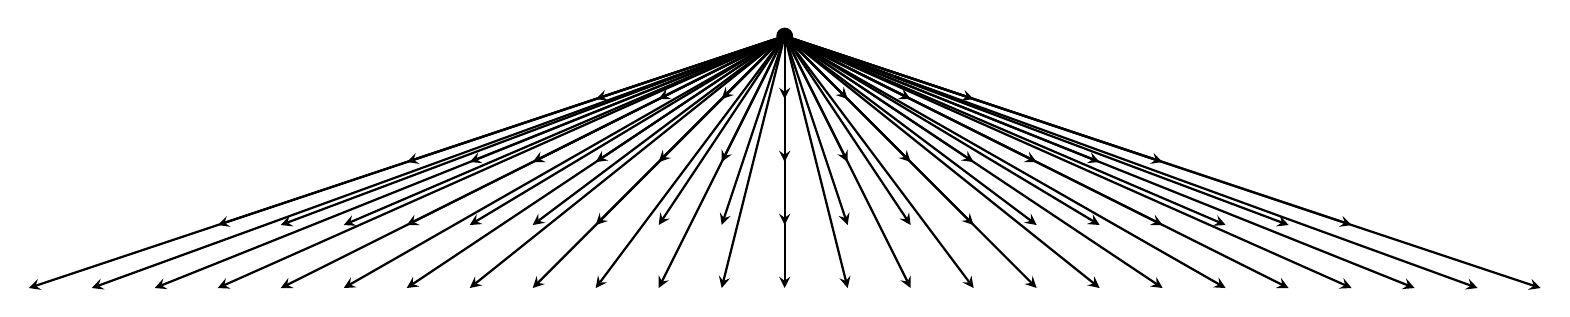
\begin{tikzpicture}[scale=0.8]
  % Root node
  \node[node] (root) at (0,4) {};

  % Level 1 branches
  \foreach \x in {-3,-2,-1,0,1,2,3} {
    \draw[branch] (root) -- (\x,3);
  }

  % Level 2 branches
  \foreach \x in {-6,-5,-4,-3,-2,-1,0,1,2,3,4,5,6} {
    \draw[branch] (root) -- (\x,2);
  }

  % Level 3 branches
  \foreach \x in {-9,-8,-7,-6,-5,-4,-3,-2,-1,0,1,2,3,4,5,6,7,8,9} {
    \draw[branch] (root) -- (\x,1);
  }

  % Level 4 branches
  \foreach \x in {-12,-11,-10,-9,-8,-7,-6,-5,-4,-3,-2,-1,0,1,2,3,4,5,6,7,8,9,10,11,12} {
    \draw[branch] (root) -- (\x,0);
  }
\end{tikzpicture}
\end{document}